\documentclass[5p,sort&compress]{elsarticle}

\usepackage{amssymb}    % Mathematical symbols
\usepackage{amsmath}    % More options for mathematics
\usepackage{subfigure}  % More options for figures
\usepackage{epstopdf}   % Convert eps to pdf
\usepackage[separate-uncertainty=true]{siunitx}   % Proper formatting of units in math mode
\usepackage{color}      % Supports text color if needed
\usepackage{soul}       % https://ctan.org/pkg/soul
\usepackage{lmodern}    % Loading fonts
\usepackage{hyperref}   % To insert clickable references/urls
\usepackage{listings}   % To input code in the text
\usepackage{amsmath}
\usepackage{amsmath}
\usepackage{amssymb}
\usepackage{graphicx}
\usepackage{epstopdf}
\usepackage{booktabs}
\setlength{\parskip}{2em}
\newcommand{\stirlingii}{\genfrac{\{}{\}}{0pt}{}}

% Choose the style of the reference list (do not change)
\bibliographystyle{elsarticle-num}

\journal{ifding/learning-notes}

% Begin the document

\begin{document}

\begin{frontmatter}
    \title{Chatper 3: Linear Models for Regression and Classification}
    \author{ifding}
    
    \begin{abstract}
        Linear Basis Function Models, The Bias-Variance Decomposition, Discriminant Functions, Probabilistic Generative Models
    \end{abstract}


\end{frontmatter}

%% How to make a heading and divide the documents into different sections
The goal of regression is to predict the value of one or more continuous \textit{target} variables \textit{t} given the value of a $D$-dimensional vector \textbf{x} of \textit{input} variables. From a probabilistic perspective, we aim to model the predictive distribution $p(t|\mathbf{x})$ because this expresses our uncertainty about the value of t for each value of \textbf{x}.

The goal in classification is to take an input vector $\boldsymbol{x}$ ans to assign it to one of K discrete classes $\mathcal{C}_k$ where $k=1, \ldots, K$. The input space is divided into \textit{decision regions} whose boundaries are called \textit{decision boundaries} or \textit{decision surfaces}. For the targe variable $\boldsymbol{t}$, it is convenient to use a 1-of-K coding scheme.


\section{Linear Basis Function Models}

Consider linear combinations of fixed nonlinear functions of the input variables,
\begin{equation}
y(\mathbf{x}, \mathbf{w})=w_{0}+\sum_{j=1}^{M-1} w_{j} \phi_{j}(\mathbf{x})
\end{equation}
where $\phi_{j}(\mathbf{x})$ are known as \textit{basis functions}. The total number of parameters in this model will be M. It is often convenient to define an additional dummy `basis function' $\phi_{0}(\mathbf{x}) = 1$.
\begin{equation}
y(\mathbf{x}, \mathbf{w})=\sum_{j=0}^{M-1} w_{j} \phi_{j}(\mathbf{x})=\mathbf{w}^{\mathrm{T}} \boldsymbol{\phi}(\mathbf{x})
\end{equation}
where $\mathbf{w} = (w_0, \ldots, w_{M-1})^{\mathrm{T}}$ and $\boldsymbol{\phi} = (\phi_0, \ldots, \phi_{M-1})^{\mathrm{T}}$. If the original variables comprise the vector $\textbf{x}$, the nonlinear basis functions $\{\phi_{j}(\mathbf{x})\}$ express the extracted features.


\subsection{Maximum likelihood and least squares}

We assume that the target variable \textit{t} is given by a deterministic function $y(\mathbf{x},\mathbf{w})$ with additive Gaussian noise so that
\begin{equation}
t=y(\mathbf{x}, \mathbf{w})+\epsilon
\end{equation}
where $\epsilon$ is a zero mean Gaussian random variable with precision (inverse variance) $\beta$. Thus we can write

\begin{equation}
p(t | \mathbf{x}, \mathbf{w}, \beta)=\mathcal{N}\left(t | y(\mathbf{x}, \mathbf{w}), \beta^{-1}\right)
\end{equation}

If we assume a squared loss function, then the optimal prediction, for a new value of \textbf{x}, will be given by the conditional mean of the target variable. In the case of a Gaussian conditional distribution, the conditional mean will be simply
\begin{equation}
\mathbb{E}[t | \mathbf{x}]=\int t p(t | \mathbf{x}) \mathrm{d} t=y(\mathbf{x}, \mathbf{w})
\end{equation}
Note hat the Gaussian noise assumption implies that the conditional distribution of t given \textbf{x} is unimodal, which may be inappropriate for some applications.


\section{The Bias-Variance Decomposition}

Although  the regularization terms can control over-fitting for models, how to determine a suitable regularization coefficient $\lambda$? What's the \textit{bias-variance} trade-off?

Given the conditional distribution $p(t | \mathbf{x})$, a popular choice is the squared loss function, for which the optimal prediction is given by the conditional expectation, $h(x)$,
\begin{equation}
h(\mathbf{x})=\mathbb{E}[t | \mathbf{x}]=\int t p(t | \mathbf{x}) \mathrm{d} t
\end{equation}

The expected squared loss can be written in the form
\begin{equation}\begin{aligned}
\mathbb{E}[L]= & \\
\int\{y(\mathbf{x})-h(\mathbf{x})\}^{2} p(\mathbf{x}) \mathrm{d} \mathbf{x}+  \int\{h(\mathbf{x})-t\}^{2} p(\mathbf{x}, t) \mathrm{d} \mathbf{x} \mathrm{d} t
\end{aligned}
\end{equation}
The second term arises from the intrinsic noise on the data and represents the minimum achievable value of the expected loss. The first term depends on our choice for the function $y(\mathbf{x})$, and we will seek a solution for $y(\mathbf{x})$ which makes this term a minimum. For a particular data set \begin{equation}
\begin{aligned}{\mathbb{E}_{\mathcal{D}}\left[\{y(\mathbf{x} ; \mathcal{D})-h(\mathbf{x})\}^{2}\right] =} \\ {\underbrace{\left\{\mathbb{E}_{\mathcal{D}}[y(\mathbf{x} ; \mathcal{D})]-h(\mathbf{x})\right\}^{2}}_{(\text {bias })^{2}}+\underbrace{\mathbb{E}_{\mathcal{D}}\left[\left\{y(\mathbf{x} ; \mathcal{D})-\mathbb{E}_{\mathcal{D}}[y(\mathbf{x} ; \mathcal{D})]\right\}^{2}\right]}_{\text {variance }}}\end{aligned}
\end{equation}
The squared \textit{bias} represents the extent to which the average prediction over all data sets differs from the desired regression function. The \textit{variance} measures the extent to which the solutions for individual data sets vary around their average, and hence this measures the extent to which the function $y(\mathbf{x} ; \mathcal{D})$ is sensitive to the particular choice of data set.

\begin{figure}[ht]
     \centering
     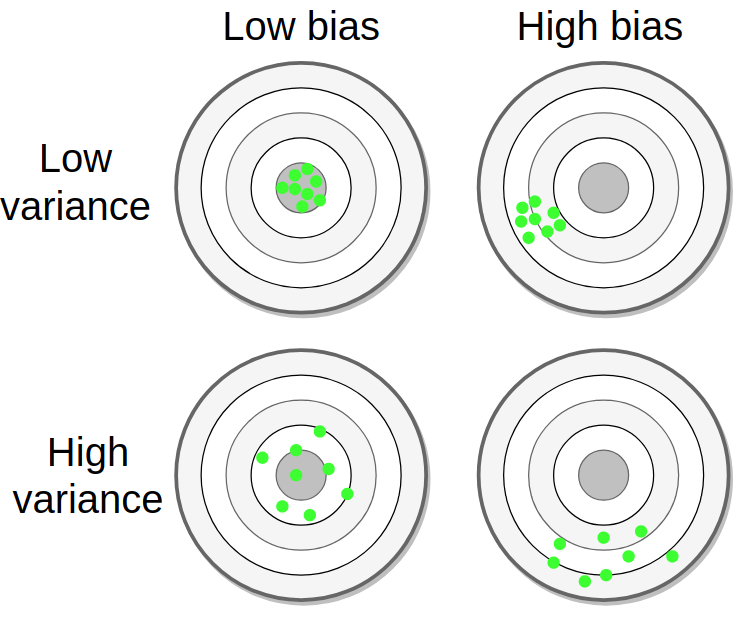
\includegraphics[width = \linewidth]{figure/bias-variance-tradeoff.png}
     \caption{The bias-variance tradeoff.}
     \label{fig:tradeoff}
\end{figure}

The decomposition of the expected squared loss
\begin{equation}
\text { expected loss }=(\text { bias })^{2}+\text { variance }+\text { noise }
\end{equation}
where
\begin{equation}
\begin{aligned}(\text { bias })^{2} &=\int\left\{\mathbb{E}_{\mathcal{D}}[y(\mathbf{x} ; \mathcal{D})]-h(\mathbf{x})\right\}^{2} p(\mathbf{x}) \mathrm{d} \mathbf{x} \\ \text { variance } &=\int \mathbb{E}_{\mathcal{D}}\left[\left\{y(\mathbf{x} ; \mathcal{D})-\mathbb{E}_{\mathcal{D}}[y(\mathbf{x} ; \mathcal{D})]\right\}^{2}\right] p(\mathbf{x}) \mathrm{d} \mathbf{x} \\ \text { noise } &=\int\{h(\mathbf{x})-t\}^{2} p(\mathbf{x}, t) \mathrm{d} \mathbf{x} \mathrm{d} t \end{aligned}
\end{equation}
There is a trade-off between bias and variance, with very flexible models having low bias and high variance, and relatively rigid models having high bias and low variance, as shown in Figure~\ref{fig:tradeoff}.


\section{Discriminant Functions}

A discriminant is a function that takes an input vector $\boldsymbol{x}$ and assigns it to one of K classes, denoted $\mathcal{C}_k$. This section focuses on \textit{linear discriminants} of two classes.

\begin{equation}
y(\mathbf{x})=\mathbf{w}^{\mathrm{T}} \mathbf{x}+w_{0}
\end{equation}
where $\mathbf{w}$ is called a \textit{weight vector}, and $w_0$ is a \textit{bias}. An input vector $\mathbf{x}$ is assigned to class $\mathcal{C}_1$ if $y(\mathbf{x}) \leq 0$ and to class $\mathcal{C}_2$ otherwise. The decision boundary is $y(\mathbf{x}) = 0$. Consider two points $\mathbf{x}_A$ and $\mathbf{x}_B$, $y(\mathbf{x}_A) = y(\mathbf{x}_B) = 0$, we have $\mathbf{w}^{\mathrm{T}} (\mathbf{x}_A -\mathbf{x}_B) = 0$ and hence the vector $\mathbf{w}$ is orthogonal to every vector lying within the decision surface.



\section{Probabilistic Generative Models}

Consider first of all the classes. The posterior probability for class $\mathcal{C}_1$ can be written as
\begin{equation}
\begin{aligned} p\left(\mathcal{C}_{1} | \mathbf{x}\right) &=\frac{p\left(\mathbf{x} | \mathcal{C}_{1}\right) p\left(\mathcal{C}_{1}\right)}{p\left(\mathbf{x} | \mathcal{C}_{1}\right) p\left(\mathcal{C}_{1}\right)+p\left(\mathbf{x} | \mathcal{C}_{2}\right) p\left(\mathcal{C}_{2}\right)} \\ &=\frac{1}{1+\exp (-a)}=\sigma(a) \end{aligned}
\end{equation}
where we have defined 
\begin{equation}
a=\ln \frac{p\left(\mathbf{x} | \mathcal{C}_{1}\right) p\left(\mathcal{C}_{1}\right)}{p\left(\mathbf{x} | \mathcal{C}_{2}\right) p\left(\mathcal{C}_{2}\right)}
\end{equation}
For the case of $K > 2$ classes, we have
\begin{equation}
\begin{aligned} p\left(\mathcal{C}_{k} | \mathbf{x}\right) &=\frac{p\left(\mathbf{x} | \mathcal{C}_{k}\right) p\left(\mathcal{C}_{k}\right)}{\sum_{j} p\left(\mathbf{x} | \mathcal{C}_{j}\right) p\left(\mathcal{C}_{j}\right)} \\ &=\frac{\exp \left(a_{k}\right)}{\sum_{j} \exp \left(a_{j}\right)} \end{aligned}
\end{equation}
which is known as the \textit{normalized exponential} and is also known as the \textit{softmax function}, as it represents a smoothed version of the `max' function because if $a_k \gg a_j$ for all $j \neq k$, then $p(\mathcal{C}_k|\mathbf{x}) \simeq 1$, and $p(\mathcal{C}_j|\mathbf{x}) \simeq 0$. Here the quantities $a_k$ are defined by
\begin{equation}
a_{k}=\ln p\left(\mathbf{x} | \mathcal{C}_{k}\right) p\left(\mathcal{C}_{k}\right)
\end{equation}


\subsection{Continuous inputs}

Let us assume that the class-conditional densities are Gaussian and all classes share the same covariance matrix.
\begin{equation}
\begin{aligned}
p\left(\mathbf{x} | \mathcal{C}_{k}\right)= \\
\frac{1}{(2 \pi)^{D / 2}} \frac{1}{|\mathbf{\Sigma}|^{1 / 2}} \exp \left\{-\frac{1}{2}\left(\mathbf{x}-\boldsymbol{\mu}_{k}\right)^{\mathrm{T}} \mathbf{\Sigma}^{-1}\left(\mathbf{x}-\boldsymbol{\mu}_{k}\right)\right\}
\end{aligned}
\end{equation}
Consider first the case of two classes.
\begin{equation}
p\left(\mathcal{C}_{1} | \mathbf{x}\right)=\sigma\left(\mathbf{w}^{\mathrm{T}} \mathbf{x}+w_{0}\right)
\end{equation}
where we have defined
\begin{equation}
\mathbf{w}=\mathbf{\Sigma}^{-1}\left(\boldsymbol{\mu}_{1}-\boldsymbol{\mu}_{2}\right)
\end{equation}
\begin{equation}
w_{0}=-\frac{1}{2} \boldsymbol{\mu}_{1}^{\mathrm{T}} \mathbf{\Sigma}^{-1} \boldsymbol{\mu}_{1}+\frac{1}{2} \boldsymbol{\mu}_{2}^{\mathrm{T}} \mathbf{\Sigma}^{-1} \boldsymbol{\mu}_{2}+\ln \frac{p\left(\mathcal{C}_{1}\right)}{p\left(\mathcal{C}_{2}\right)}
\end{equation}
The decision boundaries are linear in input space. The prior probabilities $p(\mathcal{C}_k)$ enter only through the bias $w_0$ so that changes in the priors have the effect of making parallel shits of the decision boundary.


\subsection{Maximum likelihood solution}

Suppose we have a data set $\{\mathbf{x}_n, t_n\}$ where $n = 1, \ldots, N$. Here $t_n = 1$ denotes class $\mathcal{C}_1$ and $t_n=0$ denotes class $\mathcal{C}_2$. We denote the prior class probability $p(\mathcal{C}_1) = \pi$, so that $p(\mathcal{C}_2) = 1 - \pi$. All classes share the same covariance matrix. For a data point $\mathbf{x}_n$ from class $\mathcal{C}_1$, we have $t_n = 1$ and hence
\begin{equation}
p\left(\mathbf{x}_{n}, \mathcal{C}_{1}\right)=p\left(\mathcal{C}_{1}\right) p\left(\mathbf{x}_{n} | \mathcal{C}_{1}\right)=\pi \mathcal{N}\left(\mathbf{x}_{n} | \boldsymbol{\mu}_{1}, \mathbf{\Sigma}\right)
\end{equation}
Similarly for class $\mathcal{C}_2$, we have $t_n = 0$ and hence
\begin{equation}
p\left(\mathbf{x}_{n}, \mathcal{C}_{2}\right)=p\left(\mathcal{C}_{2}\right) p\left(\mathbf{x}_{n} | \mathcal{C}_{2}\right)=(1-\pi) \mathcal{N}\left(\mathbf{x}_{n} | \boldsymbol{\mu}_{2}, \mathbf{\Sigma}\right)
\end{equation}
Thus the likelihood function is given by 
\begin{equation}
\begin{aligned}
p\left(\mathbf{t} | \pi, \boldsymbol{\mu}_{1}, \boldsymbol{\mu}_{2}, \boldsymbol{\Sigma}\right)= \\
\prod_{n=1}^{N}\left[\pi \mathcal{N}\left(\mathbf{x}_{n} | \boldsymbol{\mu}_{1}, \mathbf{\Sigma}\right)\right]^{t_{n}}\left[(1-\pi) \mathcal{N}\left(\mathbf{x}_{n} | \boldsymbol{\mu}_{2}, \mathbf{\Sigma}\right)\right]^{1-t_{n}}
\end{aligned}
\end{equation}
where $\mathbf{t} = (t_1, \ldots, t_N)^{\mathrm{T}}$. It's convenient to maximize the log of the likelihood function. Consider first the maximization with respect to $\pi$. The terms in the log likelihood function that depend on $\pi$ are
\begin{equation}
\sum_{n=1}^{N}\left\{t_{n} \ln \pi+\left(1-t_{n}\right) \ln (1-\pi)\right\}
\end{equation}
Setting the derivative with respect to $\pi$ equal to zero and rearranging, we obtain
\begin{equation}
\pi=\frac{1}{N} \sum_{n=1}^{N} t_{n}=\frac{N_{1}}{N}=\frac{N_{1}}{N_{1}+N_{2}}
\end{equation}
where $N_1$ denotes the total number of data points in class $\mathcal{C}_1$, and $N_2$ denotes the total number of data points in $\mathcal{C}_2$.

Now consider the maximization with respect to $\boldsymbol{\mu}_1$. Again we can pick out of the log likelihood function those terms that depend on $\boldsymbol{\mu}_1$ giving
\begin{equation}
\begin{aligned}
\sum_{n=1}^{N} t_{n} \ln \mathcal{N}\left(\mathbf{x}_{n} | \boldsymbol{\mu}_{1}, \mathbf{\Sigma}\right)= \\
-\frac{1}{2} \sum_{n=1}^{N} t_{n}\left(\mathbf{x}_{n}-\boldsymbol{\mu}_{1}\right)^{\mathrm{T}} \boldsymbol{\Sigma}^{-1}\left(\mathbf{x}_{n}-\boldsymbol{\mu}_{1}\right)+\text { const. }
\end{aligned}
\end{equation}
Setting the derivative with respect $\boldsymbol{\mu}_1$ to zero and rearranging, we obtain
\begin{equation}
\boldsymbol{\mu}_{1}=\frac{1}{N_{1}} \sum_{n=1}^{N} t_{n} \mathbf{x}_{n}
\end{equation}
which is simply the mean of all the input vectors $\mathbf{x}_{n}$ assigned to class $\mathcal{C}_1$. The corresponding result for $\boldsymbol{\mu}_2$ is given by
\begin{equation}
\boldsymbol{\mu}_{2}=\frac{1}{N_{2}} \sum_{n=1}^{N} (1-t_{n}) \mathbf{x}_{n}
\end{equation}
which again is the mean of all the input vectors $\mathbf{x}_{n}$ assigned to class $\mathcal{C}_2$.

Finally, consider the maximum likelihood solution for the shared covariance matrix $\mathbf{\Sigma}$, we have
\begin{equation}
-\frac{N}{2} \ln |\mathbf{\Sigma}|-\frac{N}{2} \operatorname{Tr}\left\{\mathbf{\Sigma}^{-1} \mathbf{S}\right\}
\end{equation}
where we have defined
\begin{equation}
\mathbf{S}=\frac{N_{1}}{N} \mathbf{S}_{1}+\frac{N_{2}}{N} \mathbf{S}_{2}
\end{equation}
\begin{equation}
\mathbf{S}_{1}=\frac{1}{N_{1}} \sum_{n \in \mathcal{C}_{1}}\left(\mathbf{x}_{n}-\boldsymbol{\mu}_{1}\right)\left(\mathbf{x}_{n}-\boldsymbol{\mu}_{1}\right)^{\mathrm{T}}
\end{equation}
\begin{equation}
\mathbf{S}_{2}=\frac{1}{N_{2}} \sum_{n \in \mathcal{C}_{2}}\left(\mathbf{x}_{n}-\boldsymbol{\mu}_{2}\right)\left(\mathbf{x}_{n}-\boldsymbol{\mu}_{2}\right)^{\mathrm{T}}
\end{equation}
Using the standard result for the maximum likelihood solution for a Gaussian distribution, we see that $\mathbf{\Sigma} = \mathbf{S}$, which represents a weighted average of the covariance matrices associated with each of the two classes separately.



\section*{References}
\bibliography{references}

\begin{thebibliography}{9}

\bibitem{Bishop} 
Bishop, Christopher M. Pattern recognition and machine learning. springer, 2006.

\bibitem{The bias-variance tradeoff}
https://www.machinelearningtutorial.net/2017/01/26/the-bias-variance-tradeoff/

\end{thebibliography}
\end{document}